\chapter{Hệ thống và nguồn dữ liệu liên quan}
\label{Chapter2}

Chương này trình bày những hệ thống mà nhóm chúng em đã khảo sát khi xác định hướng phát triển cho Yoca, sau đó đi vào các nguồn dữ liệu đang được sử dụng. Hai góc nhìn bổ sung cho nhau: Arkham, Dune và Nansen cho thấy cách một sản phẩm phân tích on-chain tổ chức thông tin; CoinGecko, Birdeye, Helius, Mobula, Zerion và Moralis cung cấp dữ liệu để Yoca vận hành. Qua đó, chương làm rõ khoảng trống sản phẩm cùng các ràng buộc ảnh hưởng đến kiến trúc.

\section{Các hệ thống liên quan}
\label{sec:cac_he_thong_tuong_tu}

Trong giai đoạn đầu của đồ án, từ ngày 07/09/2025 đến ngày 21/09/2025, nhóm chúng em khảo sát năm nền tảng gồm Arkham Intelligence, Birdeye, CoinGecko, Dune Analytics và Nansen. Mỗi nền tảng đại diện cho một cách tiếp cận: điều tra thực thể và dòng tiền, theo dõi token theo thời gian thực, tổng hợp thị trường, truy vấn dữ liệu tùy biến hoặc phân tích nhóm ví có ảnh hưởng. Việc đặt các cách tiếp cận cạnh nhau giúp nhóm xác định những điểm phù hợp với hành trình người dùng của đề tài.

\subsection{Arkham Intelligence}

\begin{figure}[H]
    \centering
    
\includegraphics[height=1.5cm]{images/chapter2/arkm-logo.png}
    \caption{Logo nền tảng Arkham Intelligence}
    \label{fig:platform_arkham_logo}
\end{figure}

\noindent\textit{URL: \url{https://intel.arkm.com/}}

Arkham Intelligence tập trung vào việc liên kết địa chỉ blockchain với thực thể, trực quan hóa quan hệ giữa các ví và hỗ trợ truy vết dòng tiền \cite{arkham}. Nhóm chúng em đặc biệt quan tâm đến cách Arkham biến những địa chỉ khó đọc thành một mạng lưới có ngữ cảnh. Người dùng có thể bắt đầu từ một ví, theo dõi tài sản di chuyển qua các địa chỉ trung gian và quan sát mối quan hệ giữa những thực thể đã được gắn nhãn.

Cách tiếp cận này có giá trị cao đối với điều tra chuyên sâu, nhưng cũng khiến giao diện chứa nhiều thông tin và đòi hỏi người dùng hiểu mục đích của từng công cụ. Yoca không đặt mục tiêu xây dựng một cơ sở định danh thực thể có quy mô tương đương. Bài học nhóm rút ra là dữ liệu ví chỉ thực sự hữu ích khi được đặt trong ngữ cảnh; vì vậy, Yoca ưu tiên danh mục, lịch sử giao dịch, biến động tài sản và những tín hiệu hành vi có thể giải thích trực tiếp cho người dùng.

\subsection{Birdeye và CoinGecko}

\begin{figure}[H]
    \centering
    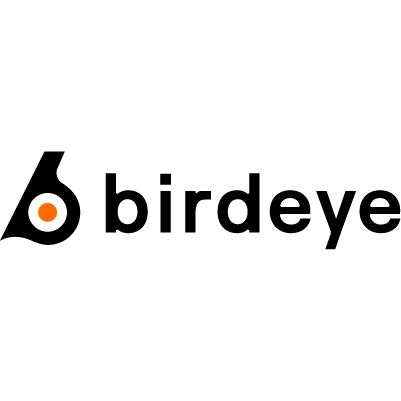
\includegraphics[height=2.5cm]{images/chapter2/birdeye-logo.png}
    \hspace{1.5cm}
    
\includegraphics[height=1.5cm]{images/chapter2/coingecko-logo.png}
    \caption{Logo nền tảng Birdeye và CoinGecko}
    \label{fig:platform_birdeye_coingecko_logo}
\end{figure}

\noindent\textit{URL: \url{https://birdeye.so/} và \url{https://www.coingecko.com/}}

Birdeye và CoinGecko cùng giúp người dùng tiếp cận dữ liệu token, nhưng có trọng tâm khác nhau. Birdeye nổi bật ở dữ liệu DEX, pool, giao dịch và biến động ngắn hạn, đặc biệt trong hệ sinh thái Solana \cite{birdeye}. CoinGecko có phạm vi thị trường rộng hơn, cung cấp danh mục coin, metadata, giá, vốn hóa, khối lượng và lịch sử thị trường trên nhiều hệ sinh thái \cite{coingecko}. Với người dùng, cả hai đều rút ngắn đáng kể quá trình tìm token, quan sát biểu đồ và đánh giá tình trạng thị trường.

Qua hai nền tảng này, nhóm chúng em nhận thấy một trang thị trường tốt cần dẫn người dùng từ thông tin tổng quan đến một token hoặc pool cụ thể. Góc nhìn thị trường sau đó được nối với phần phân tích ví để trả lời tài sản đã thay đổi như thế nào, giao dịch nào tạo ra lãi hoặc lỗ và hoạt động nào đáng chú ý.

\subsection{Dune Analytics và Nansen}

\begin{figure}[H]
    \centering
    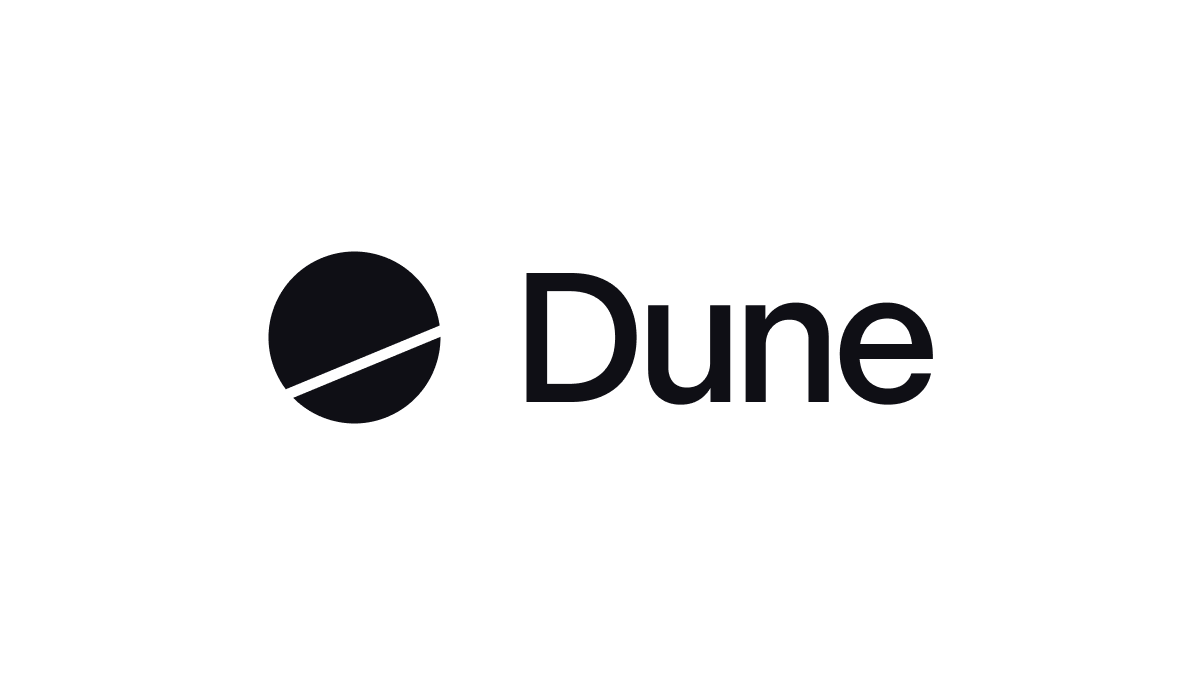
\includegraphics[height=1.5cm]{images/chapter2/dune-logo.png}
    \hspace{1.5cm}
    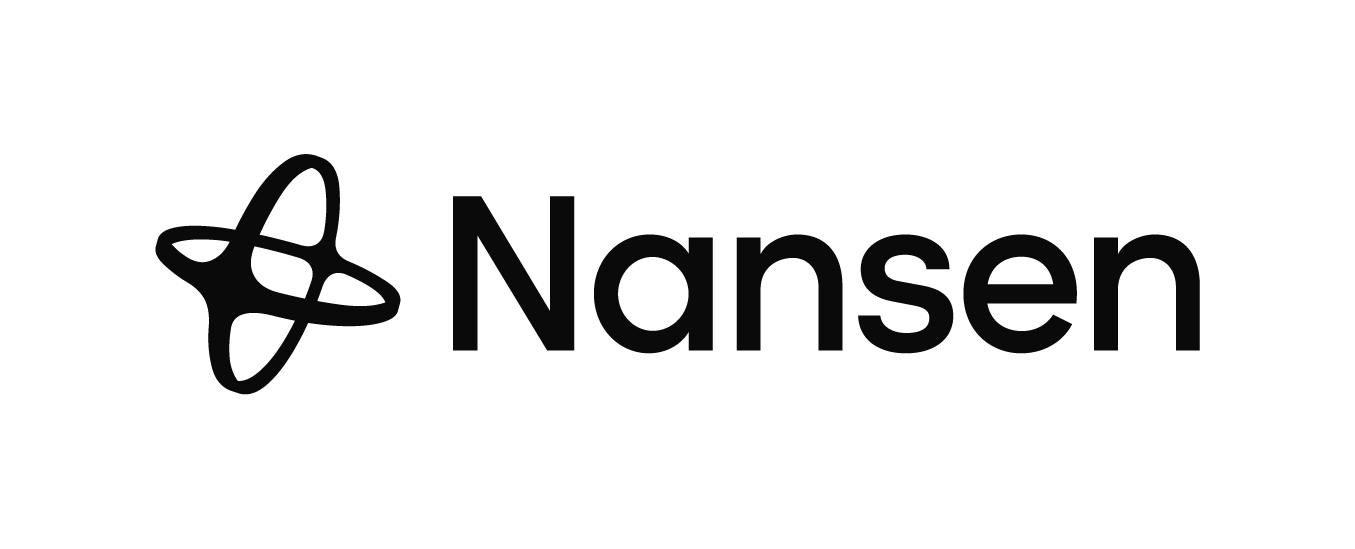
\includegraphics[height=1.5cm]{images/chapter2/nansen-logo.png}
    \caption{Logo nền tảng Dune Analytics và Nansen}
    \label{fig:platform_dune_nansen_logo}
\end{figure}

\noindent\textit{URL: \url{https://dune.com/} và \url{https://www.nansen.ai/}}

Dune Analytics cho phép cộng đồng truy vấn dữ liệu blockchain đã được lập chỉ mục và xây dựng dashboard bằng SQL \cite{dune}. Sức mạnh của Dune nằm ở khả năng tùy biến: cùng một tập dữ liệu có thể trả lời nhiều câu hỏi nghiên cứu khác nhau. Cách sử dụng này phù hợp với nhà phân tích am hiểu cấu trúc dữ liệu và SQL, nhưng tạo thêm bước chuẩn bị cho người dùng muốn xem nhanh một token hoặc ví.

Nansen tiếp cận bài toán từ dữ liệu ví đã được gắn nhãn và các nhóm hành vi như smart money \cite{nansenai}. Nền tảng làm nổi bật dòng tiền cùng hoạt động của những nhóm ví đáng chú ý, qua đó giảm công sức đọc từng giao dịch riêng lẻ. Hướng này gần với mong muốn của nhóm chúng em về việc đưa dữ liệu đã xử lý đến gần người dùng hơn, dù Nansen chủ yếu phục vụ người dùng chuyên nghiệp và dựa trên lớp dữ liệu độc quyền. Yoca lựa chọn phạm vi hẹp hơn, chuẩn bị sẵn các luồng phân tích phổ biến, duy trì khả năng kiểm chứng chỉ số nền và sử dụng AI như lớp hỗ trợ diễn giải.

\section{Đối chiếu và bài toán đặt ra cho Yoca}
\label{sec:platform_comparison_and_problem}

Các nền tảng được khảo sát không tạo thành một thang đo hơn--kém duy nhất. Arkham và Nansen có lợi thế về ngữ cảnh thực thể; Birdeye và CoinGecko mạnh ở dữ liệu thị trường; Dune trao nhiều quyền tùy biến cho người phân tích. Vì vậy, nhóm chúng em chọn các tiêu chí đối chiếu dựa trên hành trình mà Yoca muốn hỗ trợ: khám phá thị trường, đi sâu vào token hoặc pool, xem hoạt động của ví, lưu lại đối tượng quan tâm và nhận phần diễn giải dễ đọc hơn.

\begin{table}[H]
\centering
\caption{Đối chiếu định hướng của các nền tảng phân tích dữ liệu blockchain}
\label{tab:platform-comparison}
\renewcommand{\arraystretch}{1.15}
\scriptsize
\newcolumntype{Y}{>{\raggedright\arraybackslash}X}
\begin{tabularx}{\textwidth}{|p{2.3cm}|Y|Y|Y|Y|Y|}
\hline
\textbf{Tiêu chí} & \textbf{Arkham} & \textbf{Birdeye / CoinGecko} & \textbf{Dune} & \textbf{Nansen} & \textbf{Yoca} \\
\hline
Khám phá thị trường và token & Có, nhưng không phải trọng tâm & Là chức năng trọng tâm & Phụ thuộc dashboard & Có tín hiệu thị trường & Là điểm bắt đầu của luồng phân tích \\
\hline
Phân tích pool và giao dịch & Theo hướng dòng tiền & Mạnh về DEX, pool và trade & Tùy biến bằng truy vấn & Có dữ liệu đã tổng hợp & Nối pool, token và hoạt động ví \\
\hline
Phân tích ví & Mạnh về thực thể và truy vết & Có tra cứu, độ sâu tùy sản phẩm & Có thể tự xây bằng SQL & Mạnh về nhãn ví và smart money & Danh mục, PnL, lịch sử và biểu đồ ví \\
\hline
Mức độ tùy biến & Theo công cụ có sẵn & Theo màn hình và bộ lọc có sẵn & Rất cao & Theo gói phân tích có sẵn & Theo các luồng nghiệp vụ định trước \\
\hline
Khả năng tiếp cận & Thiên về điều tra dữ liệu & Dễ tiếp cận ở góc nhìn thị trường & Cần hiểu dữ liệu và truy vấn & Thiên về người dùng chuyên nghiệp & Hướng đến luồng đọc dữ liệu trực quan \\
\hline
Cá nhân hóa & Watchlist và thực thể quan tâm & Watchlist/cảnh báo tùy nền tảng & Người dùng tự xây dashboard & Theo dõi ví và nhóm nhãn & Watchlist, nhãn ví, cảnh báo và hồ sơ \\
\hline
Diễn giải dữ liệu & Ngữ cảnh thực thể & Chủ yếu trình bày chỉ số & Do tác giả dashboard quyết định & Tín hiệu được đóng gói sẵn & AI diễn giải trên dữ liệu đã kiểm chứng \\
\hline
Phát hiện hành vi bất thường & Hỗ trợ điều tra quan hệ ví & Không phải trọng tâm chung & Có thể tự xây bằng truy vấn & Có nhãn và tín hiệu chuyên sâu & Có mô-đun wash trading trong phạm vi đề tài \\
\hline
Ngôn ngữ và đơn vị hiển thị & Giao diện tiếng Anh & Giao diện tiếng Anh, giá niêm yết USD & Giao diện tiếng Anh & Giao diện tiếng Anh & Tiếng Anh và tiếng Việt, quy đổi hiển thị sang VND \\
\hline
\end{tabularx}
\end{table}

\FloatBarrier


Bảng~\ref{tab:platform-comparison} xác định phạm vi riêng của Yoca: nối các góc nhìn thường bị tách rời trong một luồng sử dụng thống nhất. Người dùng có thể bắt đầu từ tổng quan thị trường, mở pool và token liên quan, sau đó chuyển sang ví để xem danh mục, lịch sử hoạt động và kết quả phân tích. Theo dõi, cảnh báo và AI được xây dựng trên lớp dữ liệu này, trong khi số liệu nguồn vẫn được giữ để đối chiếu.

Khi hiện thực hóa luồng trên, nhóm chúng em phải kết hợp dữ liệu phân tán giữa nhiều dịch vụ. Cùng một khái niệm có thể có khóa định danh, độ sâu lịch sử và trường dữ liệu khác nhau; một phản hồi hợp lệ về mặt HTTP vẫn có thể thiếu symbol, giá hoặc phần mô tả giao dịch. Quota và chi phí của API cũng ảnh hưởng đến nhịp cập nhật, khả năng tái sử dụng dữ liệu và cách phân công nguồn. Những ràng buộc này dẫn đến lớp tích hợp provider, validation runtime, cache và các read model được trình bày trong Chương 4.

\section{Các nhà cung cấp dữ liệu được sử dụng trong Yoca}
\label{sec:data_providers}

Yoca sử dụng các API chuyên biệt cho từng miền dữ liệu rồi chuẩn hóa kết quả về mô hình nội bộ. Danh sách dưới đây phản ánh các nguồn vận hành của hệ thống tại ngày khảo sát 11/07/2026.

\subsection{Dữ liệu thị trường, token và pool}

CoinGecko là nguồn có phạm vi sử dụng rộng nhất ở miền thị trường của Yoca. Các API coin cung cấp danh sách token, metadata, tìm kiếm, giá, vốn hóa và lịch sử; nhóm Onchain DEX do GeckoTerminal cung cấp dữ liệu pool, giao dịch và tìm kiếm theo địa chỉ. CoinGecko cung cấp REST API trong cả gói Demo miễn phí và các gói trả phí; nhóm endpoint công khai bao phủ dữ liệu coin, market và một phần dữ liệu on-chain \cite{coingecko-api-docs}. Giới hạn truy vấn theo phút và phạm vi lịch sử được xử lý bằng cache cùng cơ chế tái sử dụng dữ liệu giữa các lần tương tác.

Birdeye được sử dụng cho trending token, recent trades, trader gainers/losers và một số chuỗi lịch sử giá. Trong quá trình thực hiện đề tài, nhóm chúng em sử dụng gói Lite để khảo sát các endpoint có độ sâu lịch sử lớn. Theo bảng giá tại thời điểm khảo sát, gói Standard miễn phí có phạm vi API giới hạn; gói Lite có giá 39 USD/tháng và 2,5 triệu compute unit \cite{birdeye-pricing}. Quota và chi phí vì vậy trở thành tiêu chí quan trọng khi xác định chu kỳ cache và phạm vi dữ liệu cần đồng bộ.

Mobula cũng được dùng để lấy thống kê holder của token. Tuy nhiên, vai trò quan trọng hơn của dịch vụ này nằm ở miền ví, được trình bày ở phần tiếp theo.

\subsection{Dữ liệu ví và giao dịch}

Helius là nguồn dữ liệu gắn chặt với Solana trong Yoca. Hệ thống dùng Helius Wallet API cho portfolio, lịch sử, transfer, funded-by và identity; Enhanced Transactions cung cấp giao dịch đã giải mã với token transfer, native transfer, account data và instruction \cite{helius-enhanced-transactions}. Dữ liệu này phục vụ lịch sử hoạt động, chi tiết giao dịch và webhook cảnh báo, trong khi các chỉ số PnL tổng hợp được lấy từ nguồn phân tích chuyên biệt.

Mobula là nguồn chính cho wallet analysis, PnL theo giai đoạn, vị thế theo token, lịch sử hoạt động và biểu đồ tổng giá trị ví. API cung cấp wallet activity, position, historical net worth và trading analysis trên mô hình dữ liệu đã được tổng hợp \cite{mobula-data-api}. Free tier công bố 10.000 credit/tháng; endpoint wallet analysis tiêu tốn 5 credit, còn một số endpoint wallet tính theo số chain \cite{mobula-pricing}. Yoca vì vậy lưu lại kết quả theo ví và kỳ phân tích, đồng thời giới hạn việc làm mới không cần thiết.

Zerion được sử dụng cho lịch sử số dư ở cấp token, bổ sung mức chi tiết mà chuỗi tổng tài sản từ Mobula không cung cấp. Dịch vụ có API cho portfolio, transaction, position và chart dữ liệu ví, cùng gói Developer miễn phí tại thời điểm khảo sát \cite{zerion-api}. Việc tách tổng giá trị ví và lịch sử từng token theo hai nguồn giúp mỗi biểu đồ sử dụng tập dữ liệu phù hợp với mục đích của nó.

Moralis giữ vai trò hẹp hơn, chủ yếu bổ sung metadata token và phục vụ một luồng dữ liệu swap. Dịch vụ cung cấp các nhóm Wallet, Token và Price API theo cơ chế compute unit; free tier tại thời điểm khảo sát công bố 40.000 compute unit mỗi ngày \cite{moralis-pricing}. Yoca chỉ kết hợp nhiều nguồn ở những miền có lợi ích rõ ràng, bởi khác biệt về response và semantics làm tăng chi phí duy trì schema, kiểm thử và xử lý lỗi.

\begin{table}[H]
\centering
\caption{Vai trò của các nhà cung cấp dữ liệu trong Yoca}
\label{tab:yoca_data_providers}
\renewcommand{\arraystretch}{1.2}
\scriptsize
\newcolumntype{P}{>{\raggedright\arraybackslash}X}
\begin{tabularx}{\textwidth}{|p{1.8cm}|P|P|}
\hline
\textbf{Nhà cung cấp} & \textbf{Dữ liệu Yoca đang sử dụng} & \textbf{Điểm cần kiểm soát} \\
\hline
CoinGecko & Token list, metadata, search, market, lịch sử giá, pool và pool trade & Rate limit, định danh CoinGecko và trường enrichment có thể thiếu \\
\hline
Birdeye & Trending, recent trades, trader ranking và một số lịch sử giá & Compute unit, phạm vi gói và độ sâu lịch sử của endpoint \\
\hline
Helius & Portfolio Solana, transaction, transfer, identity, funded-by và webhook & Độ sâu lịch sử và transaction abstraction không luôn đủ cho PnL \\
\hline
Mobula & Wallet analysis, PnL, position, activity, total balance history và holder & Credit theo endpoint/chain và coupling của read model phân tích ví \\
\hline
Zerion & Lịch sử số dư theo token & Sai khác trong phân loại tài sản và quota theo key \\
\hline
Moralis & Metadata token và một đường dữ liệu swap & Vai trò hẹp, chi phí duy trì nếu mở rộng thành fallback tổng quát \\
\hline
\end{tabularx}
\end{table}

Sự phân công trong Bảng~\ref{tab:yoca_data_providers} giúp mỗi miền có một nguồn ưu tiên và một mô hình dữ liệu ổn định. Provider adapter chịu trách nhiệm validation và chuẩn hóa; cache cùng read model tách giao diện khỏi cấu trúc phản hồi bên ngoài. Nhờ đó, quota, trường nullable và nhịp cập nhật của từng dịch vụ được xử lý tại biên tích hợp.

\section{Tổng kết chương}
\label{sec:tong_ket_ch2}

Qua việc khảo sát các sản phẩm hiện có, nhóm chúng em xác định Yoca tập trung vào một hành trình phân tích liền mạch, kết nối thị trường, token, pool và ví, sau đó bổ sung theo dõi và AI trên dữ liệu đã được chuẩn hóa. Điểm khác biệt của đề tài nằm ở cách các góc nhìn này hỗ trợ nhau trong cùng một trải nghiệm.

CoinGecko và Birdeye cung cấp dữ liệu thị trường; Helius cung cấp lớp dữ liệu Solana; Mobula đảm nhiệm phân tích ví; Zerion và Moralis bổ sung các miền chuyên biệt. Sự phối hợp này đặt ra yêu cầu về validation, cache và thiết kế dữ liệu, đồng thời tạo nền tảng cho các yêu cầu người dùng được trình bày ở chương tiếp theo.
